% OK!
\section{Architecture de l'application}

Dans cette partie, je vais m'attarder dans un premier temps sur l'architecture choisie pour faire le lien entre l'interface graphique de l'application et la partie \textit{business logic} (le cœur de l'application qui gère les données, les opérations avec la base de données, etc.). Dans un second temps, je présenterai l'architecture adoptée pour implémenter les exercices.

Le diagramme de classes de l'architecture du projet avec les différentes classes qui ont été utilisées est disponible en annexe \ref{appendix:class}.

\subsection{Interface graphique et \textit{business logic}}
La partie graphique de l'application et la partie \textit{business logic} doivent bien entendu être distincte. De plus, la partie \textit{business logic} doit être indépendante de la partie graphique. Cela permet, par exemple, de déployer une application web et mobile avec le même \textit{business logic}, et en définissant simplement deux interfaces différentes pour le web et le mobile.

L'architecture de l'application est un choix crucial dans le développement d'application. La modification des données par la partie \textit{business logic} doit se refléter sur la partie graphique. Un composant graphique dans le monde de \textit{Flutter} est appelé \textit{widget} (bouton, texte, layout, etc.). La programmation mobile est asynchrone et réactive, des données peuvent être modifiées par un appel réseau, par un utilisateur extérieur ou encore par un autre appareil par exemple ; les \textit{widgets} doivent réagir à ces changements.

J'ai choisi d'ajouter une couche de providers entre le niveau graphique et le \textit{business logic}. Ces providers fournissent les données nécessaires au monde graphique par l'intermédiaire de \textit{streams} (équivalent aux \textit{observables} dans \textit{ReactiveX}). Ici, un \textit{stream} peut être vu comme un tuyau unidirectionnel, le provider insère des éléments dans ce tuyau, et la partie graphique a accès à la deuxième extrémité du tuyau pour accéder à l'élément qu'il y a dans ce tuyau. Avec la famille de \textit{stream} utilisée dans l'application, chaque nouvel élément inséré dans le \textit{stream} remplace l'éventuel ancien élément.

\begin{figure}[H]
  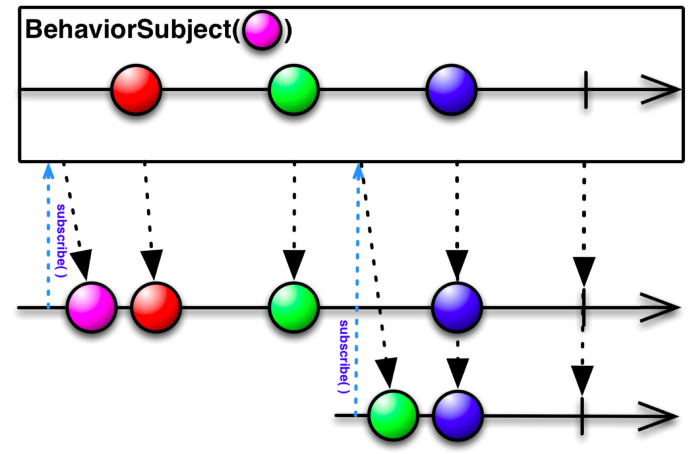
\includegraphics[width=.7\linewidth]{content/imgs/stream.png}
  \caption{Comportement des \textit{streams} des \textit{providers}}
  \label{fig:stream}
\end{figure}

Pour utiliser ces \textit{streams} dans le monde graphique, il existe le \textit{widget} \textit{StreamBuilder} qui permet d'écouter la sortie d'un \textit{stream}. Chaque nouvel élément inséré dans le \textit{stream} a pour effet de reconstruire la descendance de ce \textit{widget} : tous les fils de ce \textit{widget} seront reconstruits et redessiner à l'écran. Par exemple, si le champ texte de l'arbre de \textit{widget} de la figure \ref{fig:stream_ex1} dépend d'une donnée de la partie \textit{business logic} qui est susceptible d'être modifié au cours du temps et donc qui est disponible via un \textit{stream}, il suffit d'ajouter comme parent à ce champ texte le \textit{widget} \textit{StreamBuilder} qui va avoir accès à l'extrémité du tuyau contenant la donnée à afficher. Ce \textit{widget} et donc sa descendance (donc le champ texte) se reconstruiront automatiquement à chaque fois que le contenu du stream change (càd que le provider insère une nouvelle donnée dans le tuyau).

Cette architecture permet de reconstruire seulement les zones de l'interface graphique qui ont \textbf{besoin} d'être reconstruite suite à la modification ou à l'ajout d'une donnée (qui se passe donc dans le \textit{business logic} de l'application). C'est une architecture bien plus performante qu'une solution plus basique qui consisterait, par exemple, à reconstruire tout l'arbre de widget à partir de la racine à chaque nouveau changement.

\begin{figure}[H]
  \centering
  \begin{subfigure}{.5\textwidth}
    \centering
    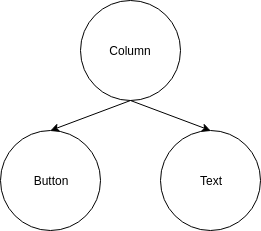
\includegraphics[width=.8\linewidth]{content/imgs/ex1.png}
    \caption{Arbre de widget composé d'un boutton et d'un texte}
    \label{fig:stream_ex1}
  \end{subfigure}%
  \begin{subfigure}{.5\textwidth}
    \centering
    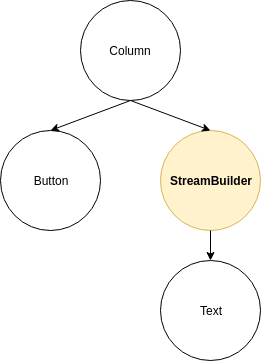
\includegraphics[width=.8\linewidth]{content/imgs/ex2.png}
    \caption{Architecture de l'arbe avec un \textit{StreamBuilder}}
  \end{subfigure}
  \caption{Exemple d'utilisation du \textit{StreamBuilder}}
\end{figure}

\subsection{Architecture des exercices}

Un aspect de l'application intéressant à concevoir était la structure des exercices. Les exercices sont différents, mais partagent tout de même beaucoup de points communs, il était donc nécessaire de trouver une architecture permettant d'implémenter différents exercices rapidement sans développer toute la base de l'exercice à chaque fois.

\begin{figure}[H]
  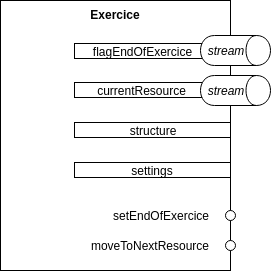
\includegraphics[width=150px]{content/imgs/exercice.png}
  \caption{Structure d'un exercice}
  \label{fig:exercice}
\end{figure}

L'architecture choisie est la suivante : un exercice possède simplement les attributs suivants :

\begin{itemize}
  \item Une \textbf{strucutre} : la liste des éléments constituant l'exercice. Plusieurs éléments peuvent être utilisés par un exercice, par exemple : un enregistreur vocal, un afficheur de mot, phrase ou texte, un métronome, etc. ;
  \item Des \textbf{réglages} : les réglages de l'exercice (choisis par l'utilisateur ou directement imposés par l'exercice). Ces réglages sont identifiés par un identifiant unique et associés à une valeur (booléen, entier, etc.) ;
  \item La \textbf{resource courrante} : la ressource actuellement utilisée par l'exercice (mot, phrase, texte) ;
  \item Un \textbf{flag} pour signaler la fin de l'exercice.
\end{itemize}

\textit{Note : pour faire simple, j'ai omis certaines informations comme la date de création, l'intitulé, etc).}

\paragraph{Structure}
Tel que vu précédemment, la structure d'un exercice est constituée de plusieurs éléments (concrètement, ces éléments sont des valeurs d'un type énuméré). Côté graphique, il y a un convertisseur de ces valeurs en un objet graphique. Par exemple, l'élément \textit{metronome} sera associé à un \textit{widget} qui affiche un métronome avec un signal visuel et un signal sonore à tempo régulier. Ces objets graphiques ont accès aux attributs et à certaines méthodes de l'exercice. Par exemple, le \textit{widget} permettant d'afficher une ressource (mot, phrase, texte), a accès à la ressource courante de l'exercice et peut appeler la fonction \texttt{moveToNextResource} pour changer la ressource courante. Ces \textit{widgets} peuvent aussi accéder aux réglages de l'exercice.

\begin{figure}[H]
  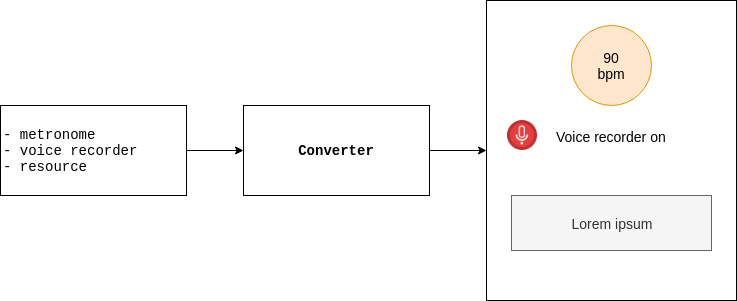
\includegraphics[width=0.8\linewidth]{content/imgs/struc.png}
  \caption{De la structure à l'interface}
  \label{fig:struc}
\end{figure}

\paragraph{Réglages}
Chaque exercice peut définir sa liste de réglages. Ces réglages sont destinés à être utilisés par les \textit{widgets} correspondant aux éléments de la structure de l'exercice. Par exemple, l'exercice du métronome peut définir le réglage \texttt{metronome\_bpm} qui va permettre au \textit{widget} affichant le métronome de régler la valeur du tempo suivant ce réglage. Comme pour les éléments de la structure des exercices, il y a un convertisseur des réglages en un objet graphique permettant de modifier les valeurs de ces réglages.

\begin{figure}[H]
  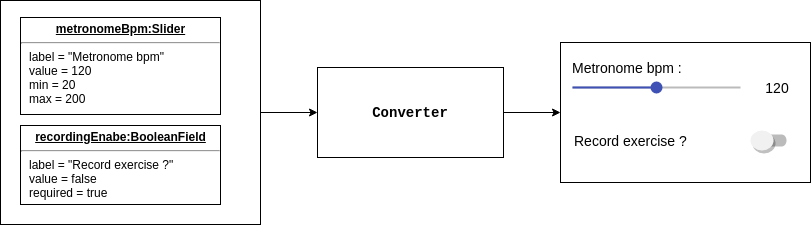
\includegraphics[width=0.8\linewidth]{content/imgs/settings.png}
  \caption{Génération visuelle des réglages de l'exercice}
  \label{fig:settings}
\end{figure}

Cette architecture permet de construire facilement et rapidement un large panel d'exercices. Pour structurer un nouvel exercice, il suffit de piocher dans la collection d'éléments déjà existante. Si un élément nécessaire à l'élaboration de l'exercice manque, il suffit alors simplement de développer ce nouvel élément pour le rajouter à la collection.






% eof
